\documentclass[3p]{elsarticle} % seleccionar: preprint, review, 1p, 3p, 5p



\usepackage{mathtools}
\journal{ }


%to force all images and table in one single section
\usepackage{placeins}
% It is necesary to add \FloatBarrier in the text. 
% After that order, all the floating are shown.

%%%%%%%%%%%%%%%%%%%%%%%
%% Elsevier bibliography styles
%%%%%%%%%%%%%%%%%%%%%%%
%% To change the style, put a % in front of the second line of the current style and
%% remove the % from the second line of the style you would like to use.
%%%%%%%%%%%%%%%%%%%%%%%

%% Numbered
%\bibliographystyle{model1-num-names}

%% Numbered without titles
%\bibliographystyle{model1a-num-names}

%% Harvard
%\bibliographystyle{model2-names.bst}\biboptions{authoryear}

%% Vancouver numbered
%\usepackage{numcompress}\bibliographystyle{model3-num-names}

%% Vancouver name/year
%\usepackage{numcompress}\bibliographystyle{model4-names}\biboptions{authoryear}

%% APA style
%\bibliographystyle{model5-names}\biboptions{authoryear}

%% AMA style
%\usepackage{numcompress}\bibliographystyle{model6-num-names}

%% `Elsevier LaTeX' style
\bibliographystyle{elsarticle-num}

%%%%%%%%%%%%%%%%%%%%%%%
\hyphenation{}
\usepackage{eurosym}
\usepackage{threeparttable} % allow the use of footnote within tables

\usepackage{url}
\usepackage[colorlinks=true, citecolor=blue, linkcolor=blue, filecolor=blue,urlcolor=blue]{hyperref}

%to add the number to the lines
\usepackage{lineno}
\modulolinenumbers[5]

\usepackage{lineno,hyperref}
\modulolinenumbers[1]
\usepackage{amsmath}
\usepackage{siunitx}
\usepackage{eurosym}
\biboptions{numbers,sort&compress}
\usepackage[europeanresistors,americaninductors]{circuitikz}
\usepackage{adjustbox}
\usepackage{xspace}
\usepackage{caption}
\usepackage{booktabs}
\usepackage{tabularx}
\usepackage{threeparttable}
\usepackage{multicol}
\usepackage{float}
\usepackage{graphicx,dblfloatfix}
\usepackage{csvsimple}
\usepackage{amsmath}
%% new commands
\newcommand{\ubar}[1]{\text{\b{$#1$}}}
\newcommand*\OK{\ding{51}}
%\renewcommand*\nompostamble{\end{multicols}}
\newcommand{\specialcell}[2][c]{%
	\begin{tabular}[#1]{@{}l@{}}#2\end{tabular}}
\def\co{CO${}_2$}
\def\el{${}_{\textrm{el}}$}
\def\th{${}_{\textrm{th}}$}


%\renewcommand*{\today}{July, 10 2018}
%\hypersetup{draft} %to avoid problems with hyperref while drafting

\begin{document}

\begin{frontmatter}

\title{Supplementary Materials for ``The benefits of ambitious short-term targets when decarbonising the European electricity and heating energy system'' }

%\author[mymainaddress,iClimate]{Marta Victoria\corref{mycorrespondingauthor}}
%\ead{mvp@eng.au.dk}
%\author[mymainaddress]{Kun Zhu}
%\author[kitaddress]{Tom Brown}
%\author[mymainaddress,iClimate]{Gorm B. Andresen}
%\author[mymainaddress,iClimate]{Martin Greiner}
%\cortext[mycorrespondingauthor]{Corresponding author}
%\address[mymainaddress]{Department of Engineering, Aarhus University, Inge Lehmanns Gade 10, 8000 Aarhus, Denmark}
%\address[iClimate]{iCLIMATE Interdisciplinary Centre for Climate Change, Aarhus University}
%\address[kitaddress]{Institute for Automation and Applied Informatics (IAI), Karlsruhe Institute of Technology (KIT), Forschungszentrum 449, 76344, Eggenstein-Leopoldshafen, Germany}



%\begin{abstract}

%\end{abstract}

%\begin{keyword}

%storage, energy system modelling, sector coupling, grid integration of renewables, transmission grid, CO2 emission targets

%\texttt{elsarticle.cls}\sep \LaTeX\sep Elsevier \sep template
%\MSC[2010] 00-01\sep  99-00
%\end{keyword}

\end{frontmatter}

\section{Historical Greenhouse Gases emissions in the European Union}

The carbon budget from now onwards for the generation of electricity and the supply of heating in residential and services sector in Europe accounts for 21 GtCO$_2$. It has been estimated based on a global carbon budget of 800 GtCO$_2$ to avoid temperature increments above 2$^{\circ}$C relative to preindustrial period with a probability of greater than 66\% \cite{Figueres_2017, blog_budget}. The global budget is assumed to be split among regions according to a constant per-capita ratio which translates into a 6\% share for Europe \cite{Raupach_2014}. Out of the total emissions in Europe, the ratio corresponding to electricity and heating is considered constant and equal to present values. In 2017, electricity generation and heating in the residential and services sector emitted 1.56 GtCO$_2$ with represents, 43.5\% of European emissions,  \cite{UNFCCC_inventory} and Figure \ref{fig_historical_emissions} . \\

\begin{figure}[!h]
\centering
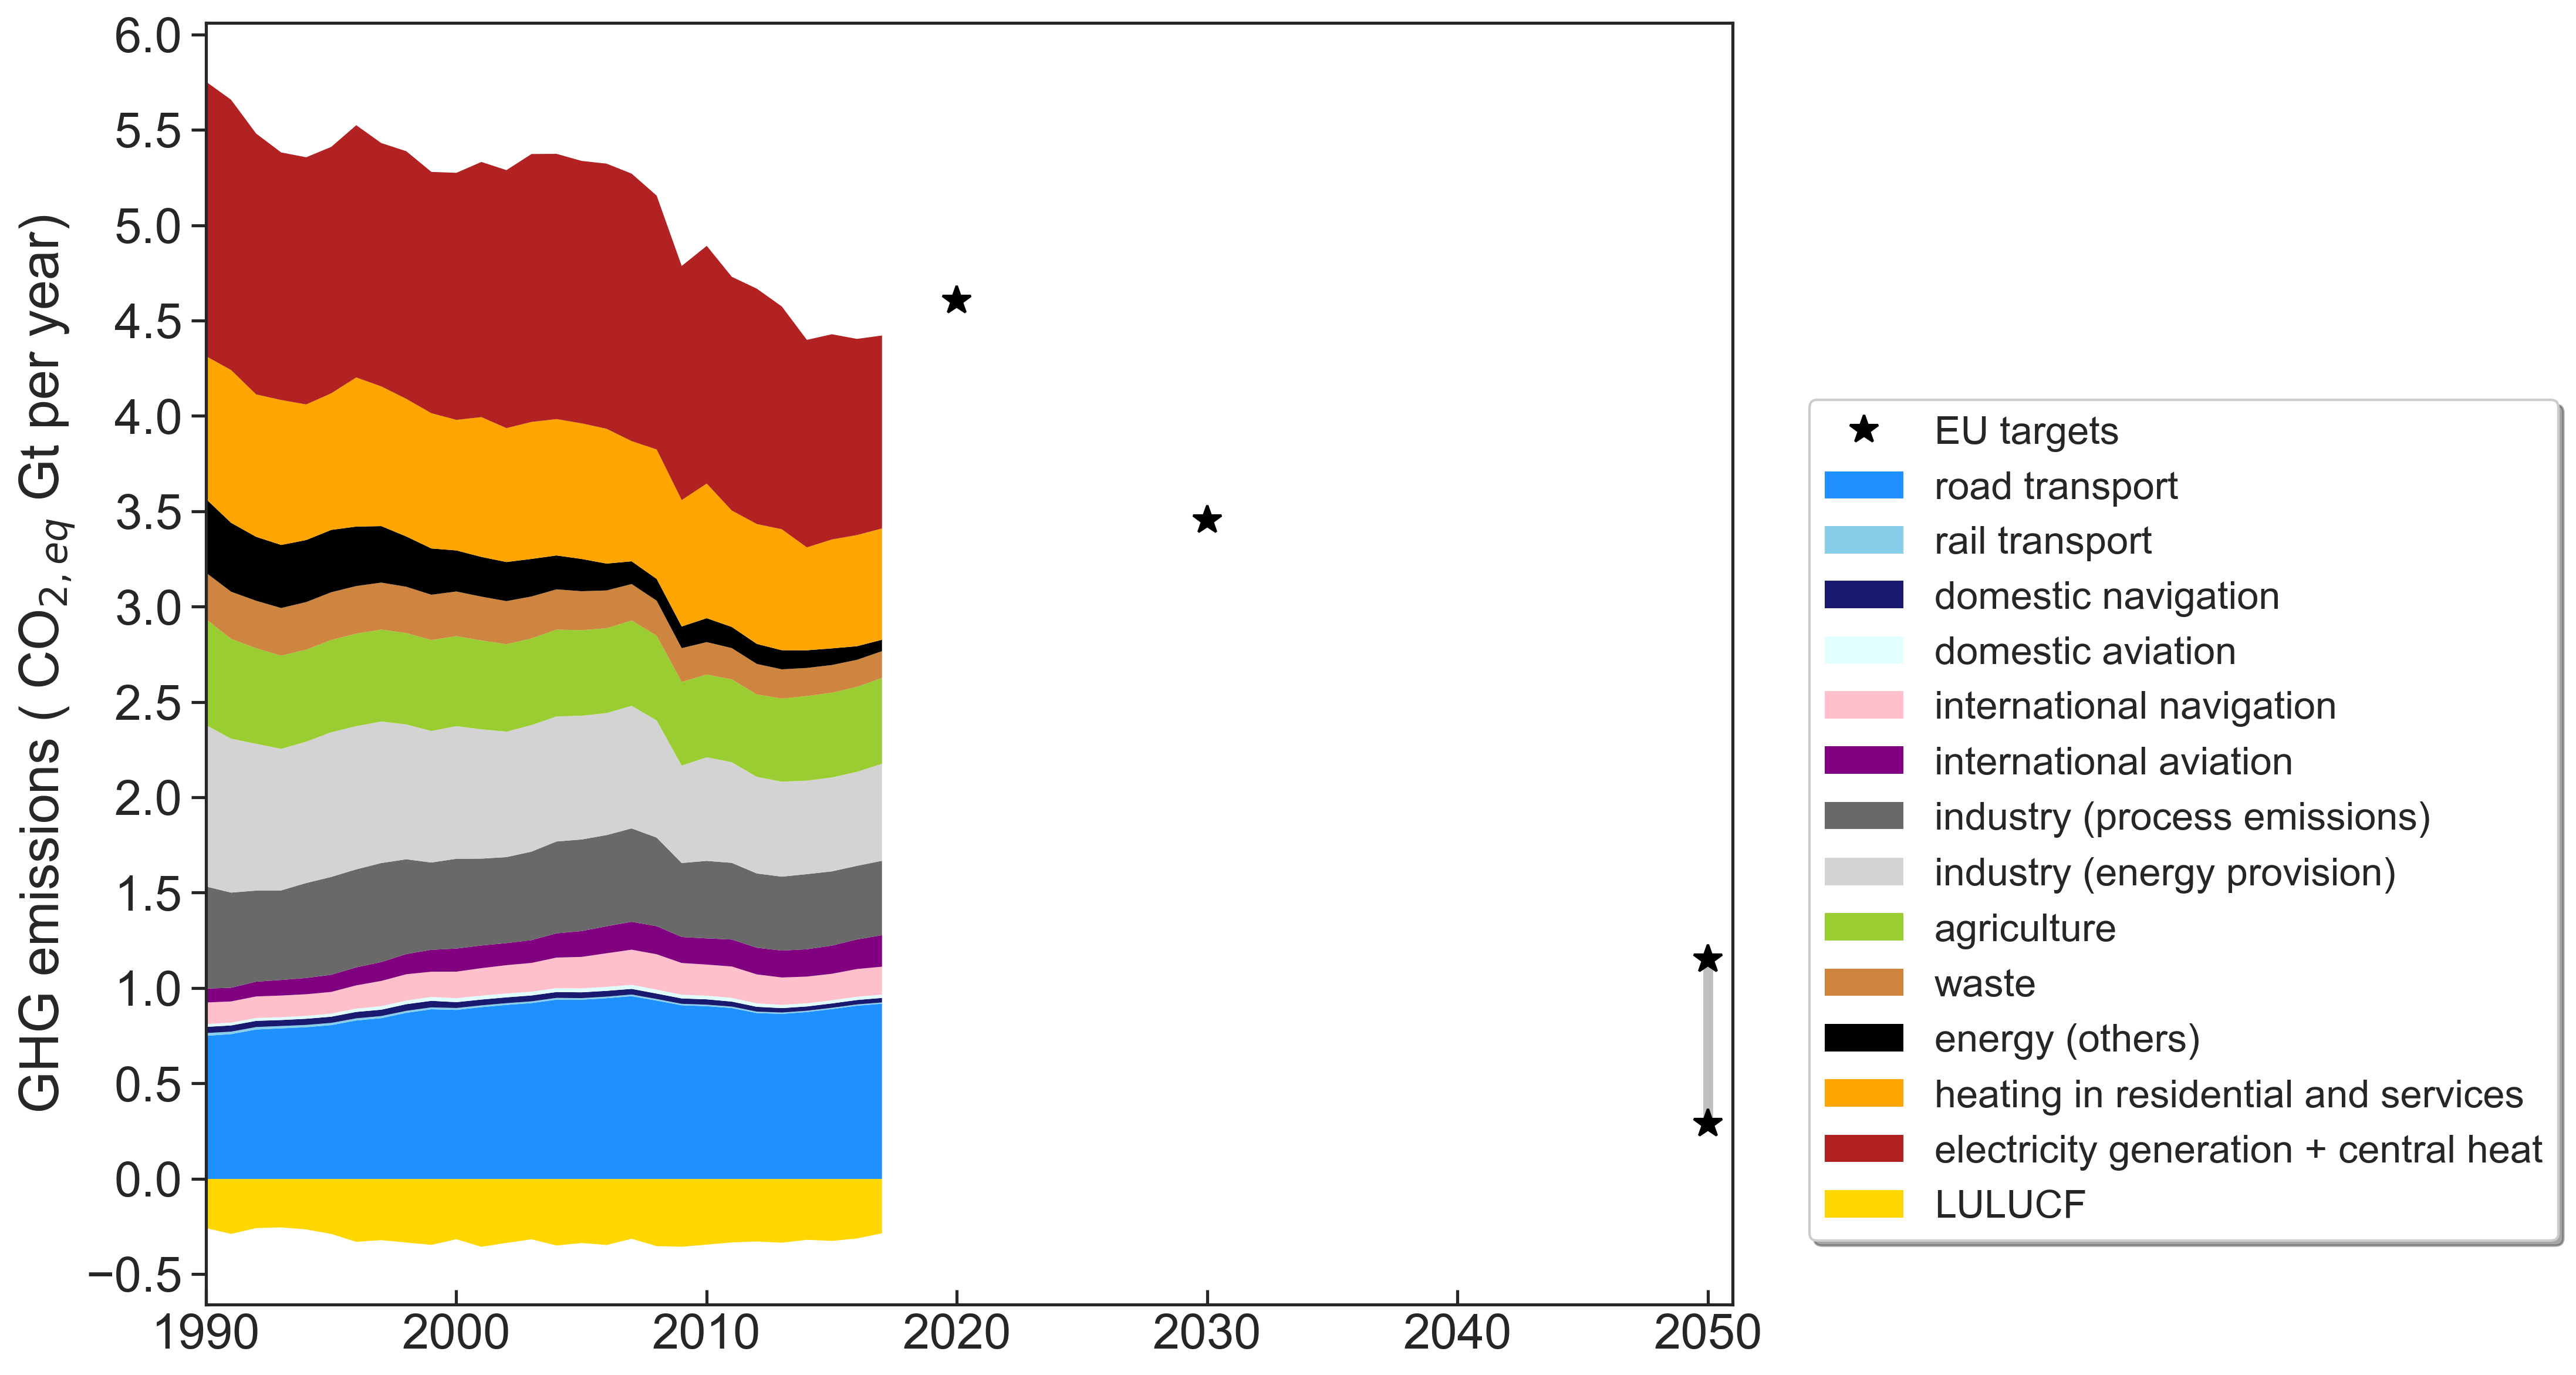
\includegraphics[width=\textwidth]{figures/historical_sectoral_emissions.png}
\caption{Sectoral distribution of historical emissions in the European Union \cite{UNFCCC_inventory}. The stars indicate committed EU reduction targets.} \label{fig_historical_emissions} 
\end{figure}

\section{CO$_2$ restriction paths with equivalent budget}

The 21 GtCO$_2$ budget $B$ can be utilised following different transition paths. One option consists in assuming a linear CO$_2$ restriction path. Emissions will then reach zero in $t_f$

\begin{equation}
	t_f=t_0+\frac{2B}{e_0}
\end{equation}

Where $t_0$=2020, and $e_0$ represents the carbon emissions from electricity and heating sector in 2020, which are assumed to be the same as in 2017. \\

Alternatively, emissions can be assumed to follow a path defined by one minus the cumulative distribution function (CDF$_\beta$) of a beta distribution in which $\beta_1$ = $\beta_2$. 

\begin{equation}
\begin{aligned}
&	e (t) = e_0(1- CDF_{\beta}(t)) \\
&	CDF_{\beta} (t) =\int_{-\infty}^{t} PDF_{\beta}(t) dt \\
&	PDF_{\beta} (t) =  \frac{\Gamma(\beta_1+\beta_2)}{\Gamma(\beta_1)+\Gamma(\beta_2)} t^{\beta_1-1} (1-t)^{\beta_2-1}
\end{aligned}
\end{equation}

where $\Gamma$ is the gamma function. The cumulative emissions fulfil $\int_{t_0}^{\infty} e(t) dt =B$. \\

The third option considered for the transition path is an exponential decay, following Raupach \textit{et al. }\cite{Raupach_2014}. In that case, emissions evolve as:
\begin{equation}
e(t) = e_0(1+(r+m)t)e^{-mt}
\end{equation}

where $r$ is the initial linear growth rate, which here is assumed to be $r$=0, and the decay parameter $m$ is determined by imposing the integral of the path to be equal to the budget.
\begin{equation}
\begin{aligned}
& B=\int_{t_0}^{\infty} e_0(1+(r+m)t)e^{-mt} dt \\
& m=\frac{1+ \sqrt{1+\frac{rB}{e_0}}}{\frac{B}{e_0}}
\end{aligned}
\end{equation}

Although the exponential decay path approaches asymptotically to zero, we assume here that $e(2050)=0$. By doing that, the final point of the different transition paths is equivalent and all of them achieve net-zero emissions by 2050.

\section{Historical evolution of CO$_2$ emissions from heating supply in residential and services sector in European countries}

\begin{figure}[!h]
\centering
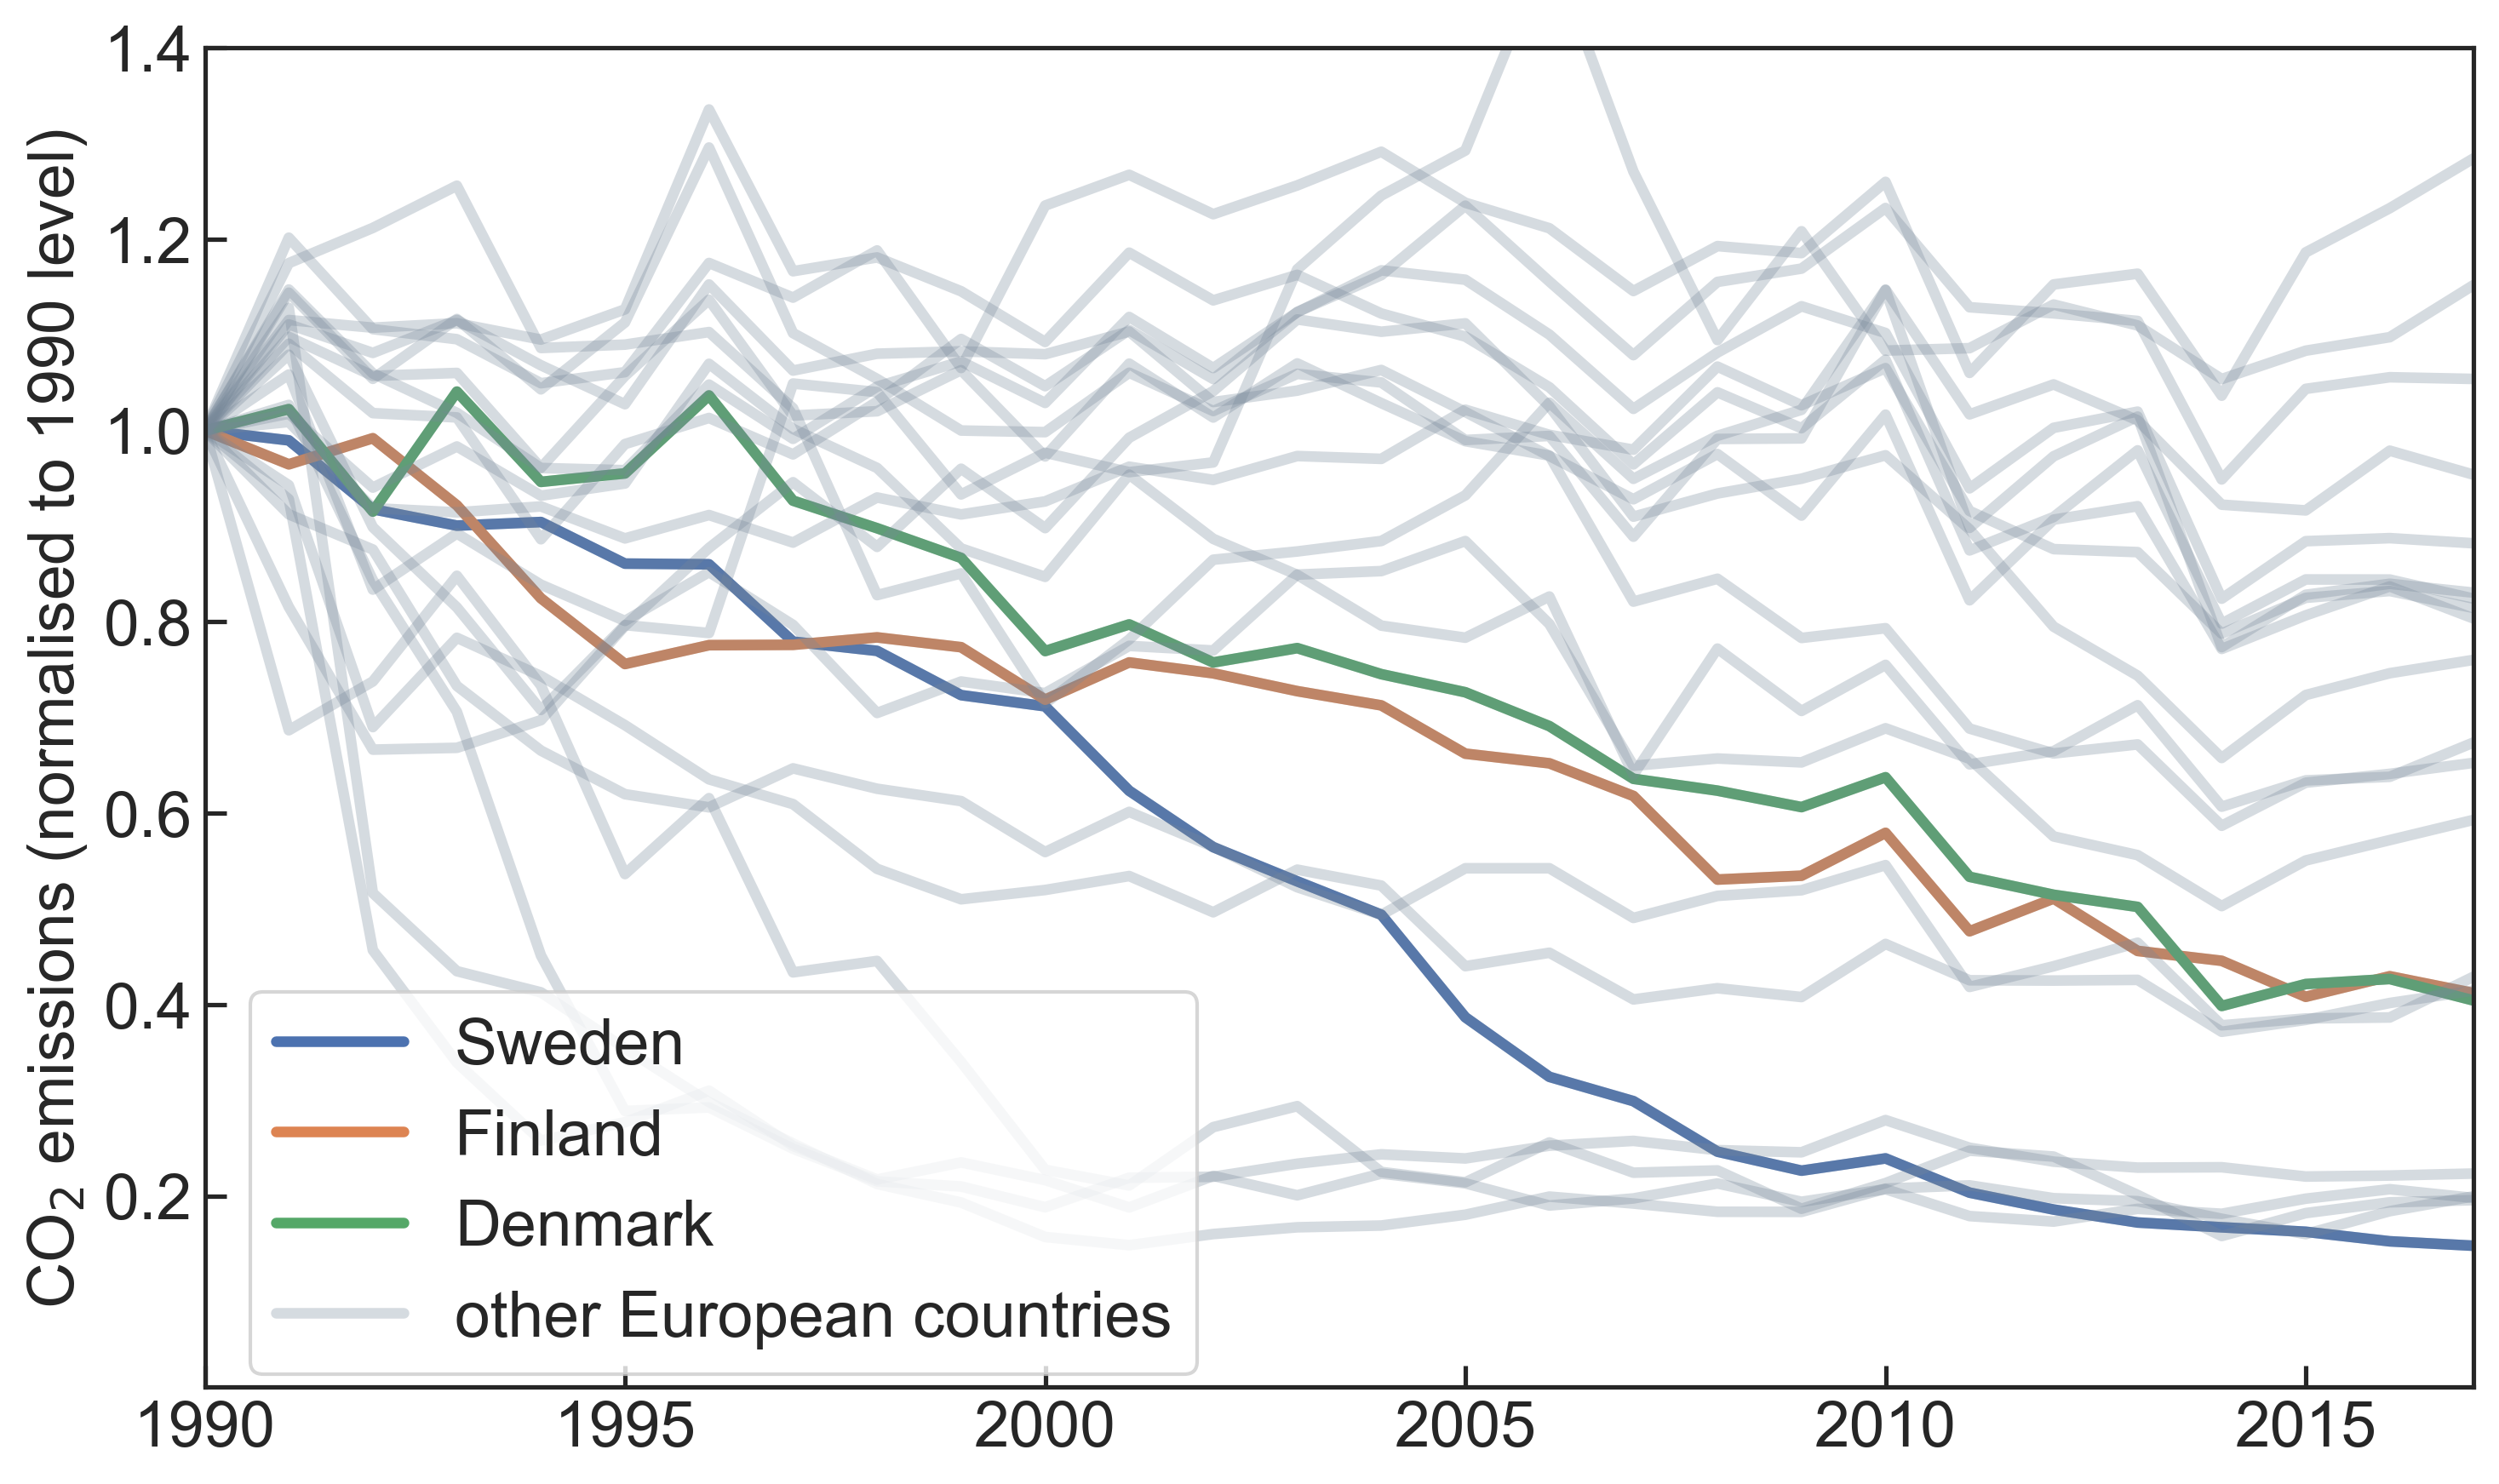
\includegraphics[width=12cm]{figures/emissions_heating.png}
\caption{Historical CO$_2$ emissions from heating in residential and services sector \cite{UNFCCC_inventory}. } \label{fig_emissions_heating} 
\end{figure}

\begin{figure}[!h]
\centering
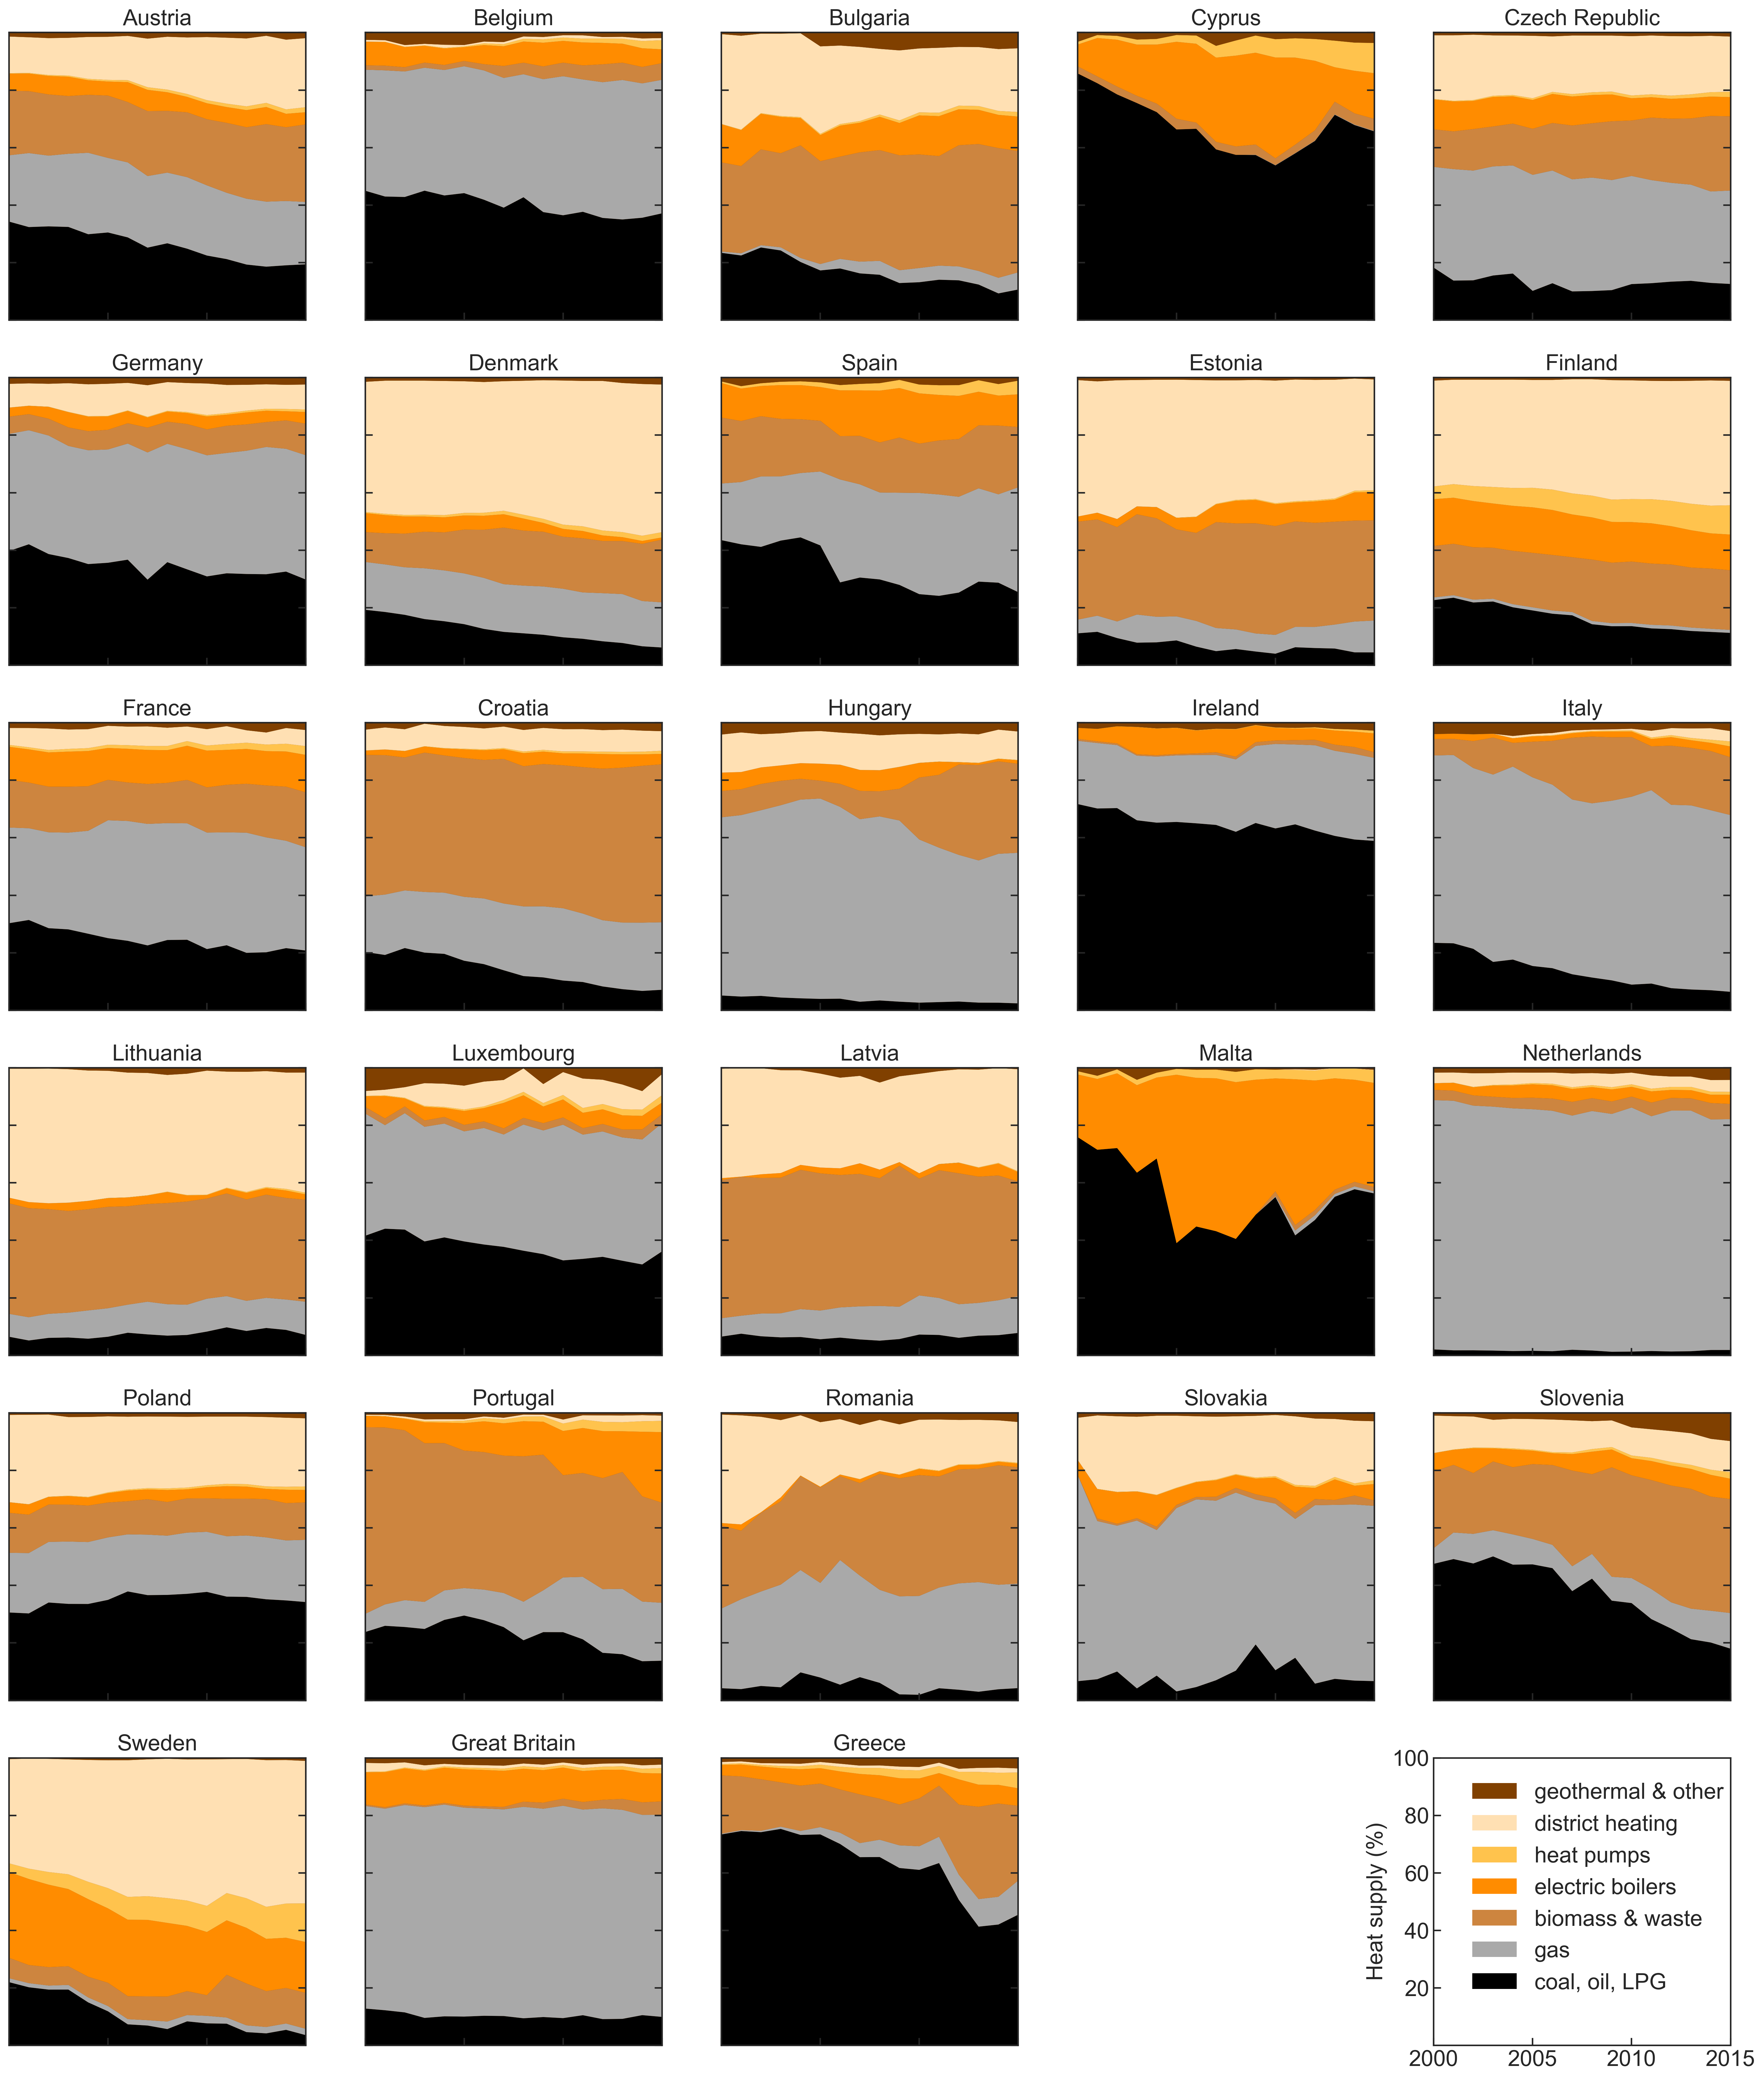
\includegraphics[width=\textwidth]{figures/heating_historical.png}
\caption{Historical share of technologies used to supply heating in residential and services sector \cite{IDEES}. } \label{fig_historical_heating} 
\end{figure}

\section{Power plants in operation in Europe}

\begin{figure}[!h]
\centering
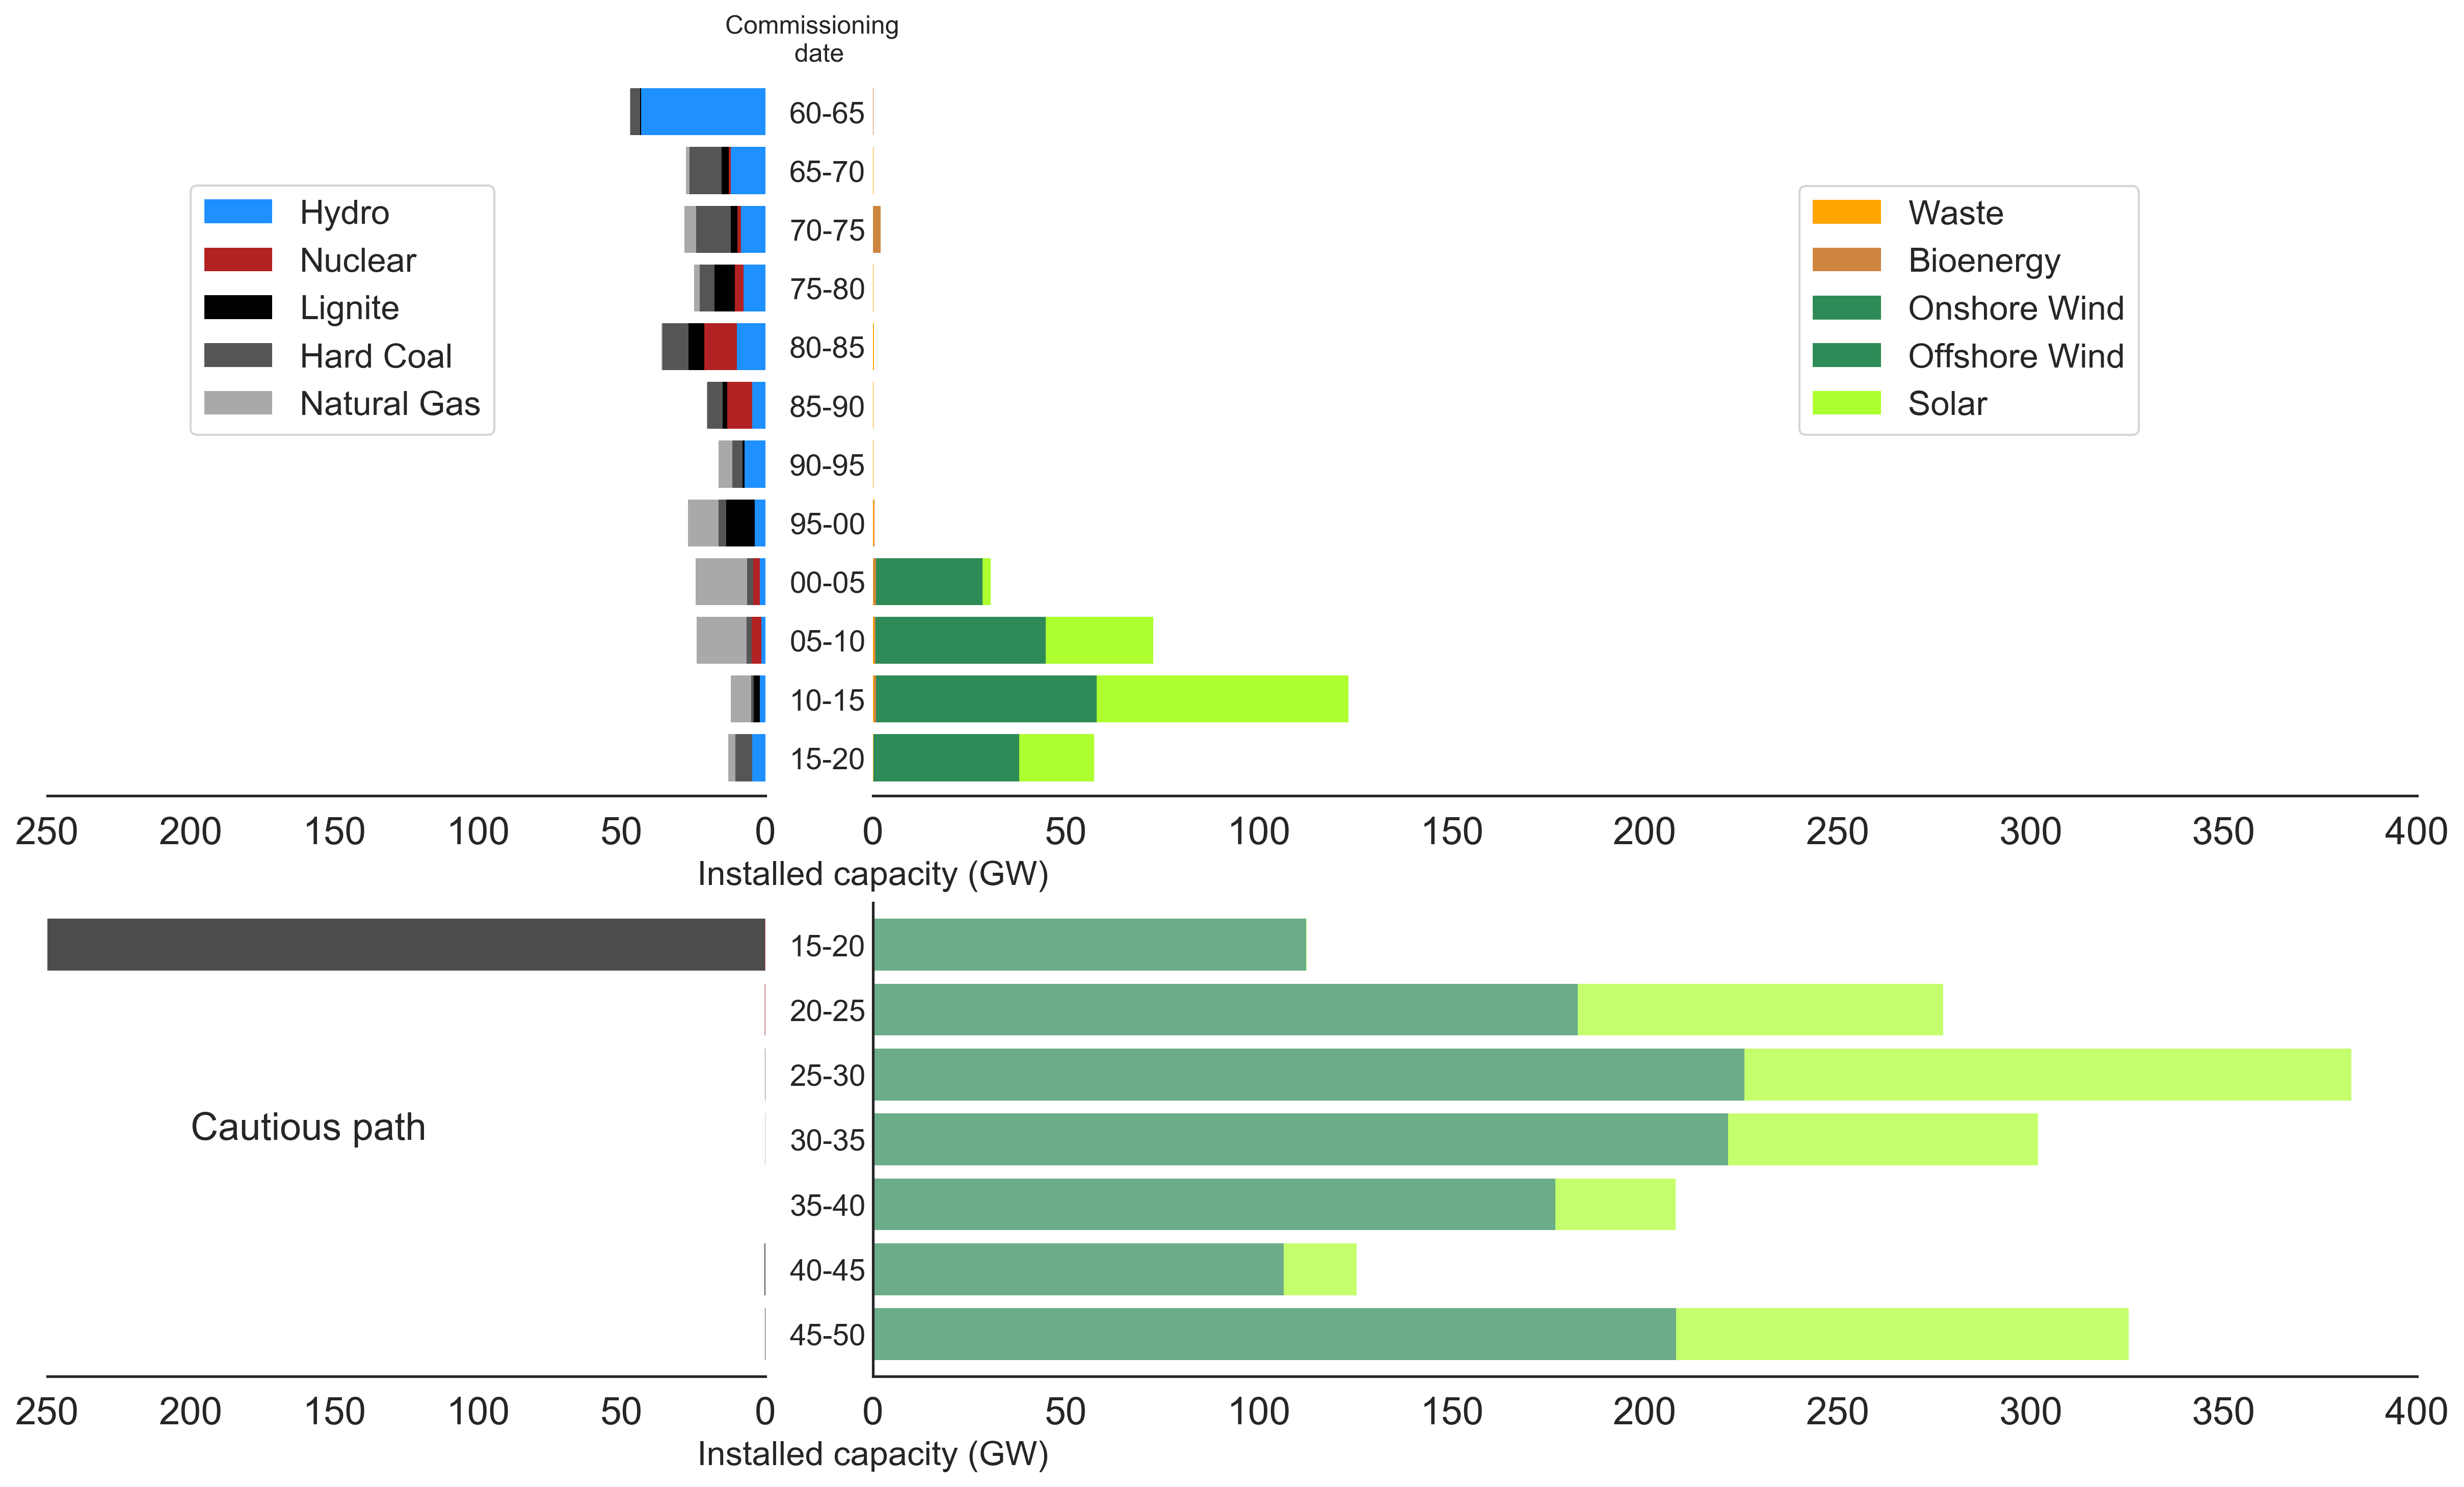
\includegraphics[width=\textwidth]{figures/age_distribution.png}
\caption{Age distribution of European power plants in operation\cite{powerplantmatching, IRENA_2019}} \label{fig_age_distribution} 
\end{figure}

\section{Historical build rates for solar photovoltaics in European countries}

\begin{figure}[!h]
\centering
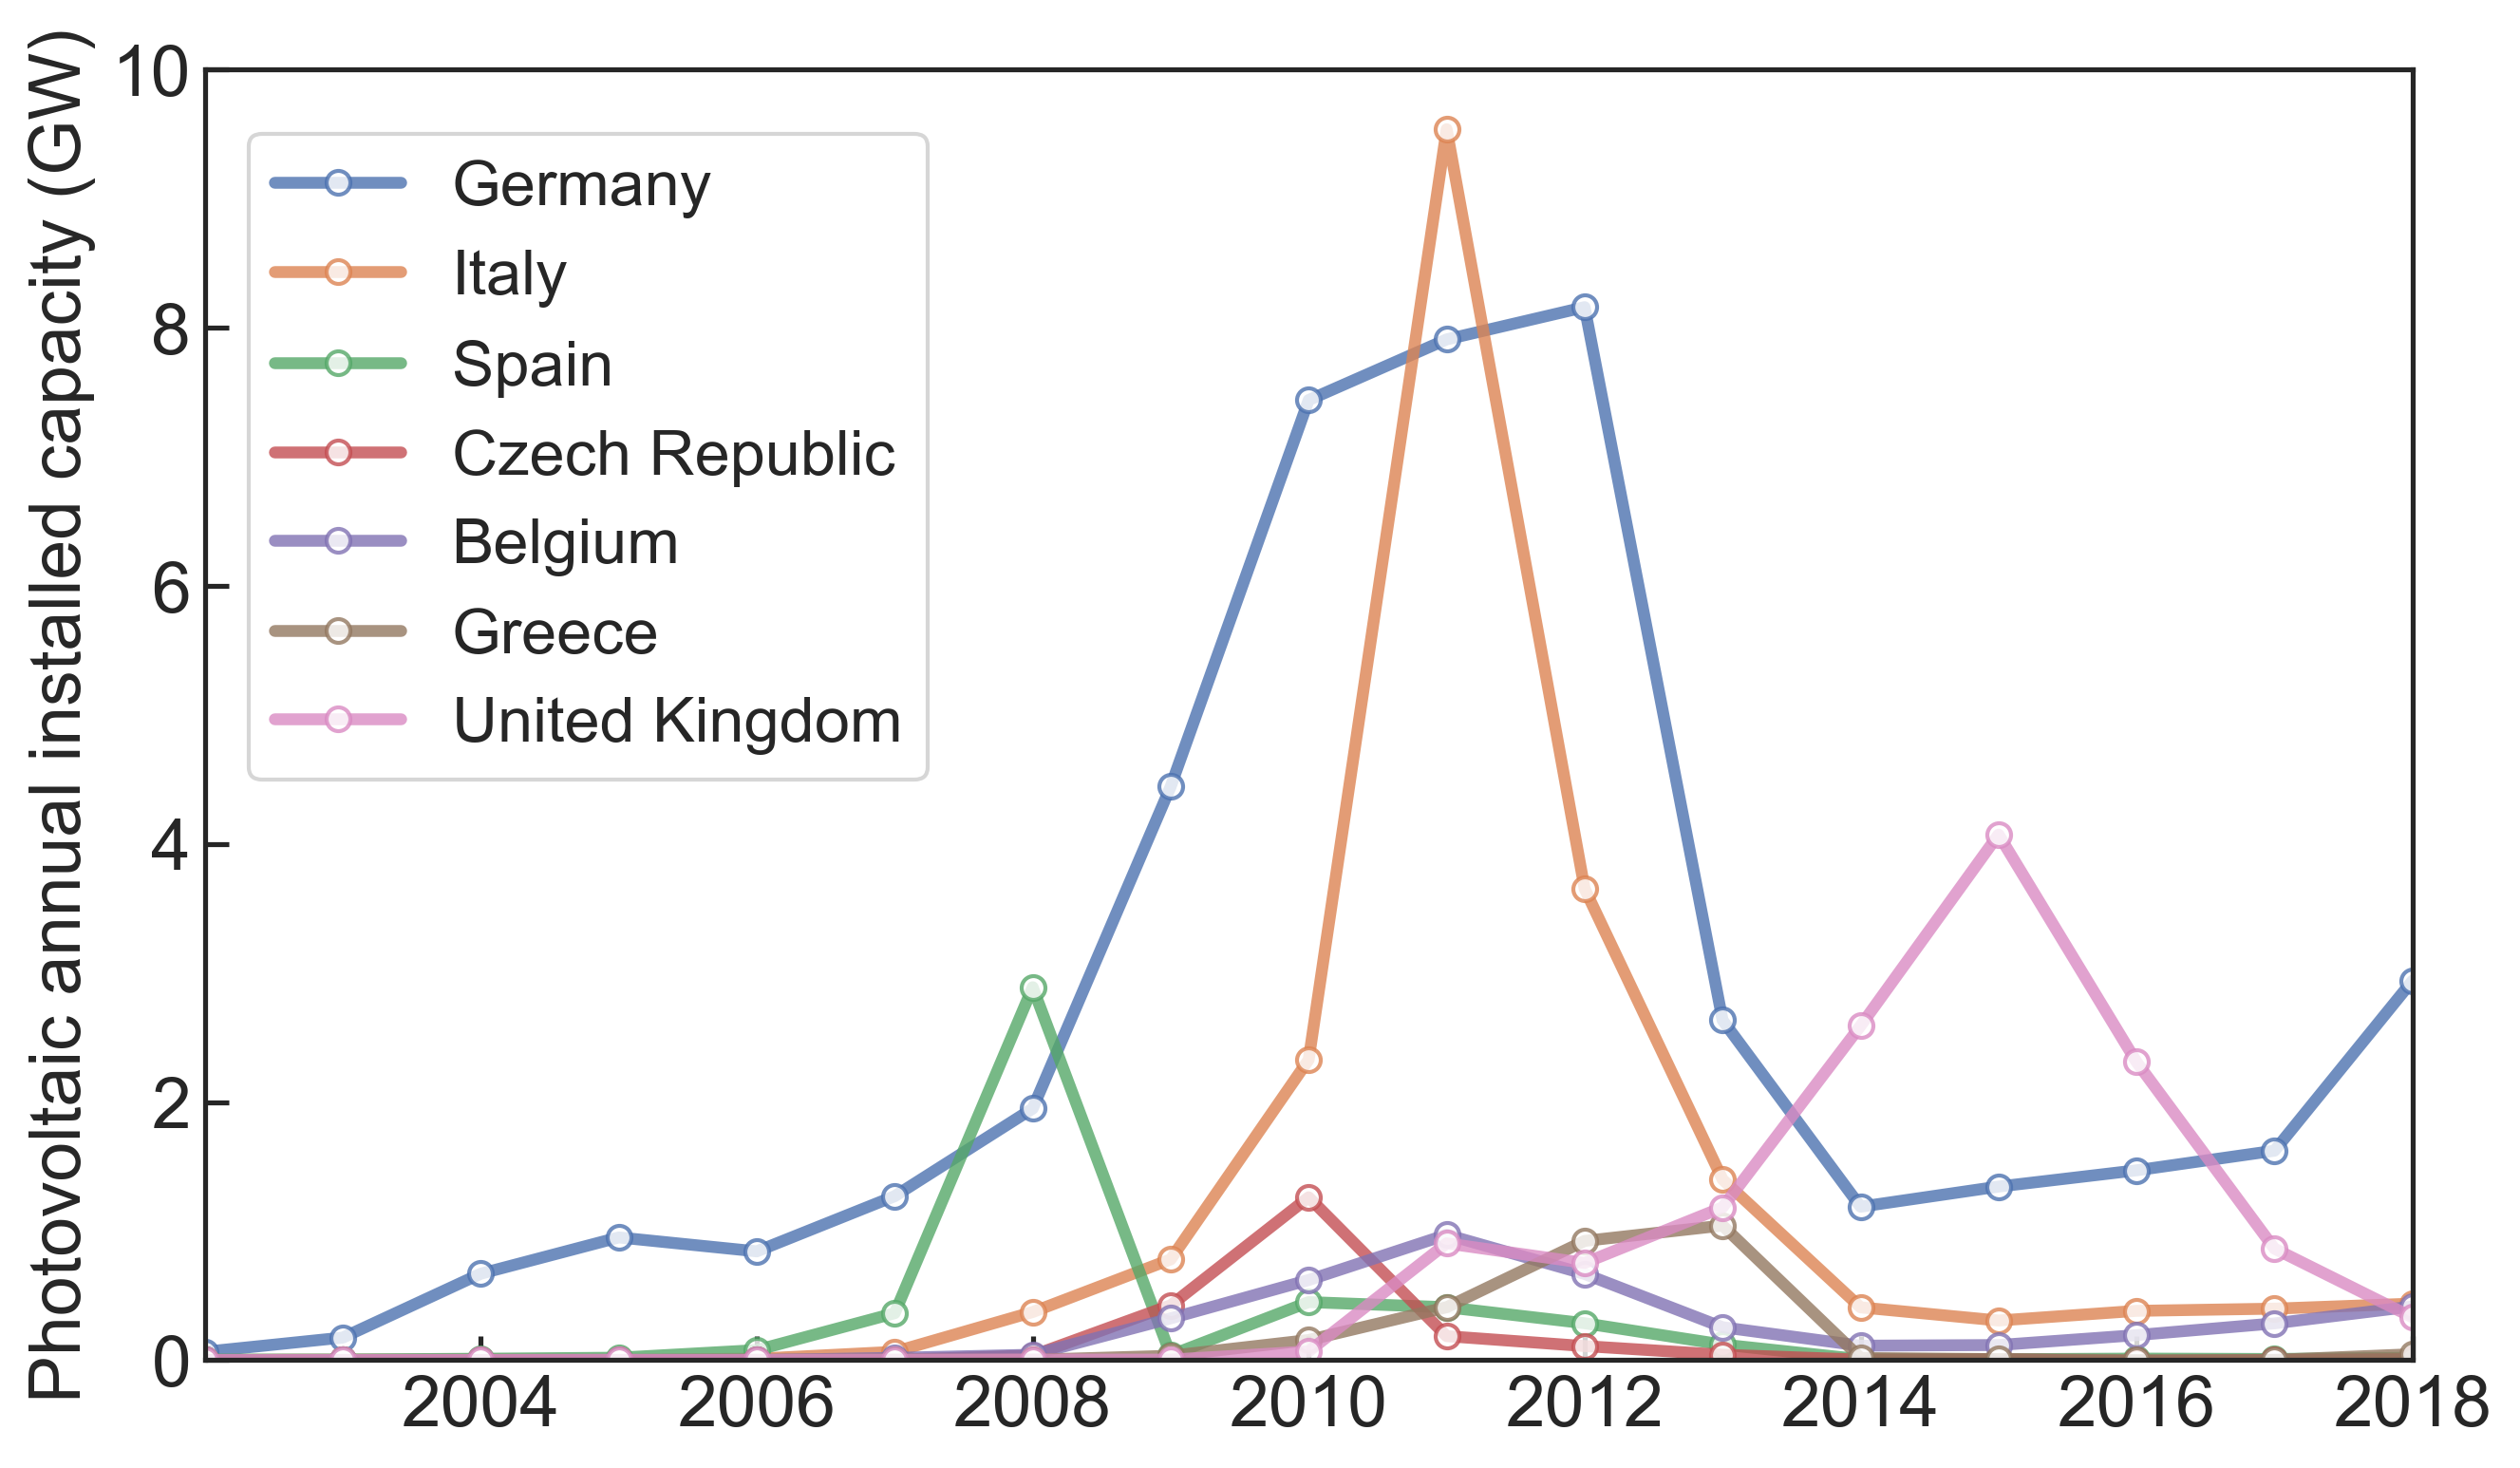
\includegraphics[width=12cm]{figures/installation_rates_PV.png}
\caption{Photovoltaic annual build rates for those European countries with a prominent peak \cite{IRENA_2019}. The sharp increase and subsequent decrease in the installation rates were caused by country-specific successive changes in the regulatory frameworks. See for instance \cite{Report_Fraunhofer_2019, Victoria_2012}. } \label{fig_installation_rates_PV} 
\end{figure}
 


\section{Transition paths cautious and last-minute. Additional results}

\begin{figure}[!h]
	\centering
	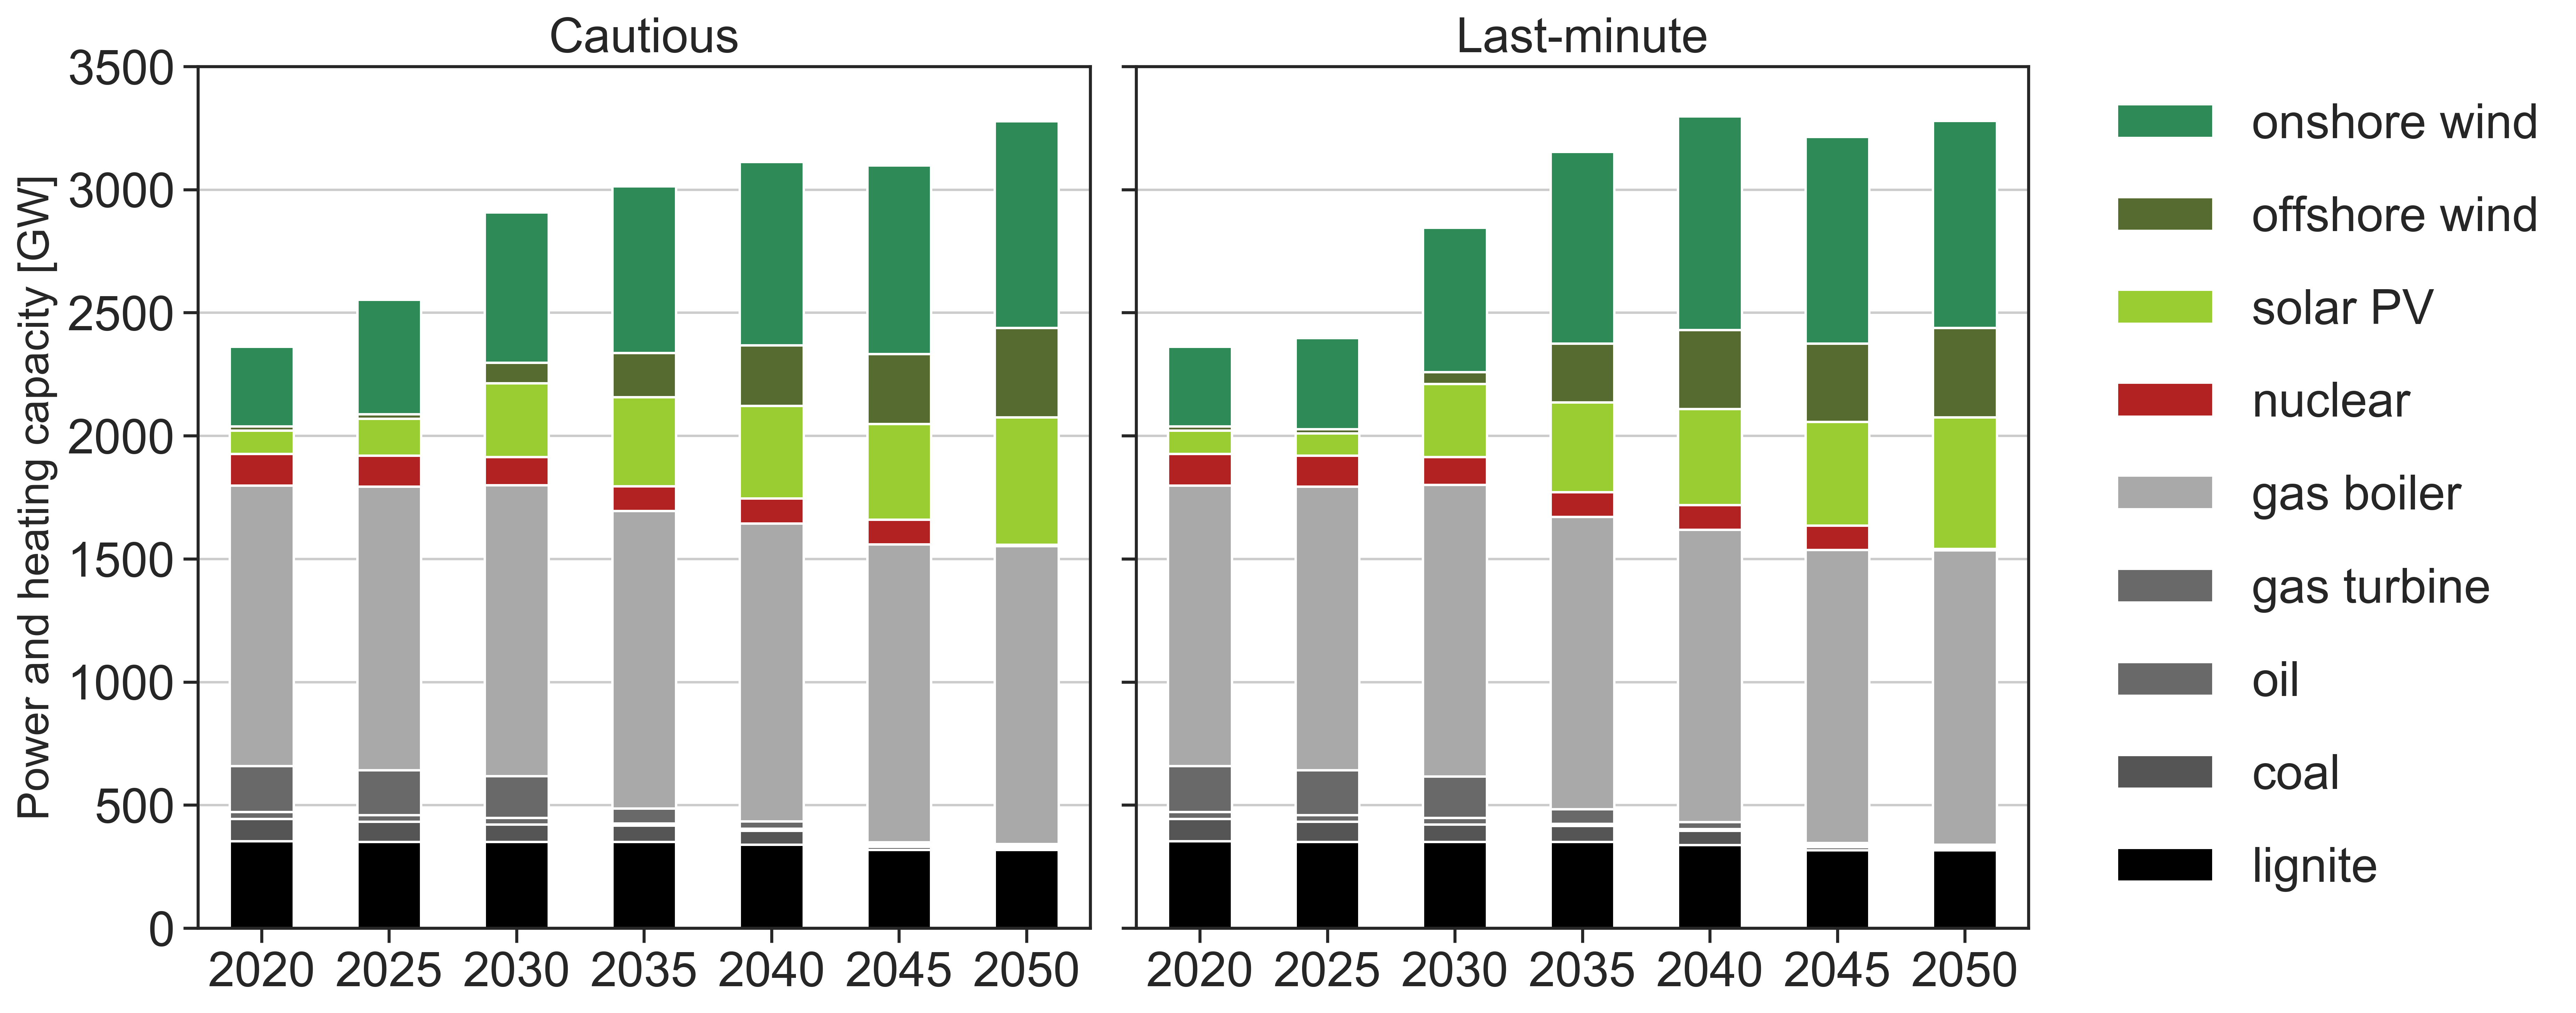
\includegraphics[width=12cm]{figures/installed_capacity.png}
	\caption{Installed capacities for different technologies throughout transition paths cautious and last-minute shown in Fig. 1 in the main text.} \label{fig_installed_capacity} 
\end{figure}

\begin{figure}[!h]
\centering
%	\includegraphics[width=\columnwidth]{figures/spatial_plot_primary_energy.png}
\caption{Primary energy in every country in 2050. (left) Cautious transition path, (right) Greenfield optimization for 2050.} \label{fig_spatial_plot} 
\end{figure}

\begin{figure}[!h]
\centering
%\includegraphics[width=\textwidth]{figures/.png}
\caption{Evolution of technologies used to supply heating in residential and services sector in the cautious path. } \label{fig_heating_shares} 
\end{figure}

\FloatBarrier

\section{Model description}

In every time step, the optimisation objective, that is, the total annualised system cost is calculated as:

\begin{align}
& \min_{\substack{G_{n,s},E_{n,s},\\F_\ell,g_{n,s,t}}} \left[ \sum_{n,s} c_{n,s} \cdot G_{n,s} +\sum_{n,s} \hat{c}_{n,s} \cdot E_{n,s} \right. \nonumber \\
& \hspace{2cm} \left. + \sum_{\ell} c_{\ell} \cdot F_{\ell}+ \sum_{n,s,t} o_{n,s,t} \cdot g_{n,s,t} \right]
\label{eq_objective}
\end{align}

where $c_{n,s}$ are the fixed annualised costs for generator and storage power capacity $G_{n,s}$ of technology $s$ in every bus $n$, $\hat{c}_{n,s}$ are the fixed annualised costs for storage energy capacity $E_{n,s}$, $c_\ell$ are the fixed annualised costs for bus connectors $F_{\ell}$, and $o_{n,s,t}$ are the variable costs (which in some cases include CO$_2$ tax), for generation and storage dispatch $g_{n,s,t}$ in every hour $t$. Bus connectors $\ell$ include transmission lines but also converters between the buses implemented in every country (see Figure \ref{Fig_buses}), for instance, heat pumps that connect the electricity and heating bus. \\

The optimisation of the system is subject to several constraints. First, hourly demand $d_{n,t}$ in every bus $n$ must be supplied by generators in that bus or imported from other buses. $f_{\ell,t}$ represents the energy flow on the link $l$ and $\alpha_{n,\ell,t}$ indicates both the direction and the efficiency of flow on the bus connectors.  $\alpha_{n,\ell,t}$ can be time dependent such as in the case of heat pumps whose conversion efficiency depends on the ambient temperature.

\begin{equation}
\sum_{s} g_{n,s,t}+ \sum_{\ell} \alpha_{n,\ell,t}\cdot f_{\ell,t} = d_{n,t} \hspace{.2cm} \leftrightarrow \hspace{0.2cm} \lambda_{n,t} \hspace{.3cm} \forall\, n,t \label{eq_energy_balance}
\end{equation}

The Lagrange multiplier $\lambda_{n,t}$,  also known as Karun-Kush-Tucker (KKT),  associated with the demand constraint indicates the marginal price of the energy carrier in the bus $n$, \textit{e.g.}, local marginal electricity price in the electricity bus. \\

Second, the maximum power flowing through the links is limited by their maximum physical capacity $F_{\ell}$. For transmission links, $\ubar{f}_{\ell,t}=-1$ and $\bar{f}_{\ell,t}=1$, which allows both import and export between neighbouring countries. For a unidirectional converter \textit{e.g.}, a heat resistor, $\ubar{f}_{\ell,t}=0$ and $\bar{f}_{\ell,t}=1$ since a heat resistor can only convert electricity into heat.

\begin{equation}
\ubar{f}_{\ell,t} \cdot F_{\ell} \leq f_{\ell,t} \leq \bar{f}_{\ell,t} \cdot F_{\ell} \hspace{1cm} \forall\, \ell,t \; . \label{eq_links}
\end{equation}

For interconnecting transmission lines, the lengths $l_{\ell}$ are set by the distance between the geographical mid-points of each country, so that some of the transmission within each country is also reflected in the optimisation. A factor of 25\% is added to the line lengths to account for the fact that transmission lines cannot be placed as the crow flies due to land use restriction. For the transmission lines capacities $F_{\ell}$, a safety margin of 33\% of the installed capacity is used to satisfy n-1 requirements \cite{Brown_2016}. \\ %Linear optimal power flow is applied using Kirchhoff's formulation \cite{Horsch_2018}. 

Third, for every hour the maximum capacity that can provide a generator or storage is bounded by the product between installed capacity $G_{n,s}$ and availabilities $\ubar{g}_{n,s,t}$, $\bar{g}_{n,s,t}$. For instance, for solar generators $\ubar{g}_{n,s,t}$ is zero and $\bar{g}_{n,s,t}$ refers to the capacity factor at time $t$ 

\begin{equation}
\ubar{g}_{n,s,t} \cdot G_{n,s} \leq g_{n,s,t} \leq \bar{g}_{n,s,t} \cdot G_{n,s} \hspace{1cm} \forall\, n,s,t \; . \label{eq_g}
\end{equation}

The maximum power capacity for generators is limited by potentials $\bar{G}_{n,s}$ that are estimated taking into account physical and environmental constraints:
\begin{equation}\label{eq_max_G}
0 \leq G_{n,s}\leq \bar{G}_{n,s} \hspace{1cm} \forall\, n,s \; .
\end{equation}

The storage technologies have a charging efficiency $\eta_{in}$ and rate $g_{n,s,t}^+$, a discharging efficiency $\eta_{out}$ and rate $g_{n,s,t}^-$, possible inflow $g_{n,s,t,\textrm{inflow}}$ and spillage $g_{n,s,t,\textrm{spillage}}$, and standing loss $\eta_0$. The state of charge $e_{n,s,t}$ of every storage has to be consistent with charging and discharging in every hour and is limited by the energy capacity of the storage $E_{n,s}$. It should be remarked that the storage energy capacity $E_{n,s}$ can be optimised independently of the storage power capacity $G_{n,s}$.

\begin{align}
e_{n,s,t} = & \ \eta_0 \cdot e_{n,s,t-1} + \eta_{in} |g_{n,s,t}^+| - \eta_{out}^{-1} |g_{n,s,t}^-| \nonumber \\
& + g_{n,s,t,\textrm{inflow}} - g_{n,s,t,\textrm{spillage}} \; , \nonumber \\
& 0  \leq   e_{n,s,t} \leq E_{n,s}   \hspace{0.5cm} \forall\, n,s,t \; . \label{eq_storage}
\end{align}

So far, equations (\ref{eq_energy_balance}) to (\ref{eq_storage}) represent mainly technical constraints but additional constraints can be imposed to bound the solution.\\

The interconnecting transmission expansion can be limited by a global constraint
\begin{equation}
\sum_{\ell} l_\ell \cdot F_{\ell} \leq  \textrm{CAP}_{LV} \hspace{.7cm} \leftrightarrow \hspace{0.3cm} \mu_{LV} \; ,
%\hspace{.3cm} 
\label{eq_cap}
\end{equation}
where the sum of transmission capacities $F_{\ell}$ multiplied by the lengths $l_{\ell}$ is bounded by a transmission volume cap $\textrm{CAP}_{LV}$. In this case, the Lagrange/KKT multiplier $\mu_{LV}$ represents the shadow price of a marginal increase in transmission volume.\\


The maximum CO$_2$ allowed to be emitted by the system $\textrm{CAP}_{CO2}$ can be imposed through the constraint 

\begin{equation}
  \sum_{n,s,t}  \varepsilon_{s} \frac{ g_{n,s,t} }{\eta_{n,s}} + \sum_{n,s} \varepsilon_{s} (e_{n,s,t=0} - e_{n,s,t=T})  \leq  \textrm{CAP}_{CO2} \hspace{.4cm} \leftrightarrow \hspace{0.3cm} \mu_{CO2} \label{eq_co2cap}
\end{equation}

where $\varepsilon_{s}$ represents the specific emissions in CO$_2$-tonne-per-MWh\th{} of the fuel $s$, $\eta_{n,s}$ the efficiency and $g_{n,s,t}$ the generators dispatch. In this case, the Lagrange/KKT multiplier represents the shadow price of CO$_2$, \textit{i.e.}, the additional price that should be added for every unit of CO$_2$ to achieve the CO$_2$ reduction target in an open market. 

\section{Sectors description and data}

\textcolor[rgb]{1,0,0}{TODO: Add data references for electricity demand and annual demand, methodology description for modelling hourly heat demand. Describe modelling approach for wind and solar PV time series and reference repositories. 
Describe temperature-dependency of heat pumps. Describe operation of CHP power plants. 
Reference data for initially installed electricity and heat generation capacities. Describe path of deployment of district heating. Describe path of electrification of transport. Include formula for LCOE estimation. }

\section{Cost assumptions}	

\begin{table*}[!b]
\begin{threeparttable}
\caption{Cost assumption per technology and year.} \label{tab:cost per year}
\centering
\begin{tabularx}{\textwidth}{l|c|c|c|c|c|c|c|r}
\toprule
Technology\tnote{1}&2020&2025&2030&2035&2040&2045&2050&source\\
\midrule
Battery inverter\\
Battery storage\\
Coal power plant\\
Combined heat and power\\
Direct air capture\\
Electric boiler\\
Electrolysis\\
Fuel cell\\
Gas boiler central\\
Gas boiler individual\\
Heat pump central\\
Heat pump individual\\
High voltage direct current line\\
Hot water tank central\\
Hot water tank individual\\
Hydro reservoir\\
Hydrogen storage\\
Lignite power plant\\
Methanation\\
Nuclear\\
Offshore wind \\
Oil power plant\\
Onshore wind \\
Open cycle gas turbine\\
Pumped hydro storage\\
Run of river\\
Solar PV rooftop\\
Solar PV utility\\
\bottomrule
\end{tabularx}
\begin{tablenotes}
\item[1] Sorted by alphabet.
\end{tablenotes}
\end{threeparttable}
\end{table*}

\begin{table}
\caption{Efficiency, lifetime and FOM cost per technology, include references.}
\end{table}

\begin{figure}[!h]
\centering
%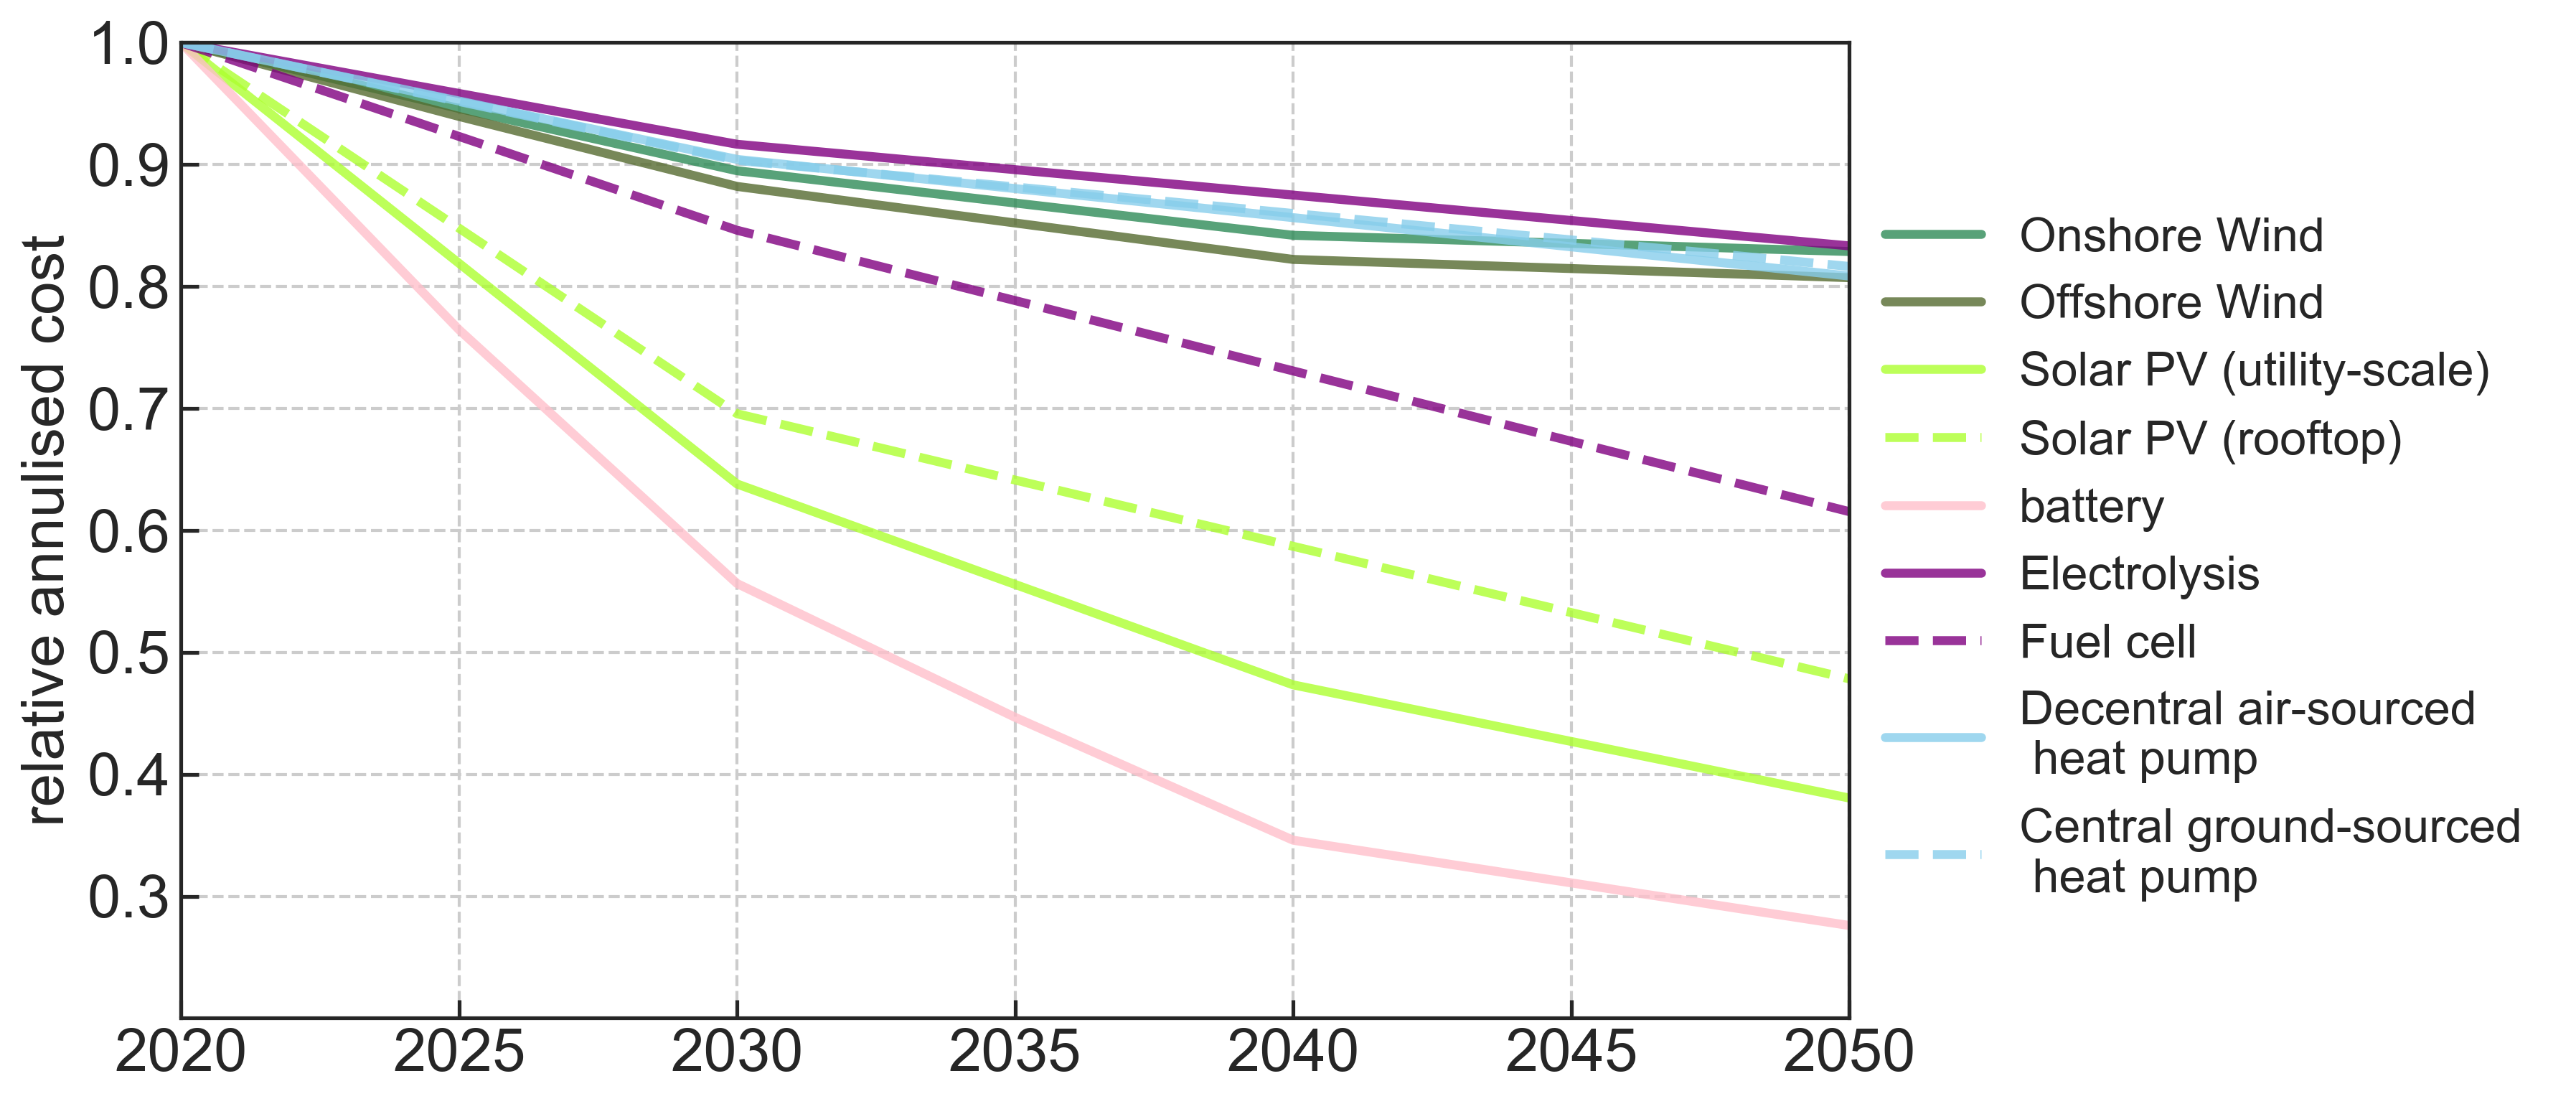
\includegraphics[width=12cm]{figures/cost_evolution.png}
\caption{Cost evolution assumed for the different technologies. } \label{fig_cost_evolution} 
\end{figure}


 
\section{References}
\bibliography{bib_transition}

\end{document}